\chapter{Resuelve ecuaciones lineales I}

\section{Ecuación lineal en una variable y función lineal}

\subsection*{Resumen}

Si $a, b$ son numéros constantes tal que $a \neq 0$, una ecuación lineal
se escribe $ax + b = 0$ donde $x$ es la incógnita. La única solución de esta
ecucación es $x = -\frac{b}{a}$.

Si $a, b$ son numéros constantes, la función $f(x) = ax + b$ es una función
lineal. El gráfico de la función $f(x) = ax + b$ es el conjunto de los puntos de
coordenadas $(x, y)$ donde $y = ax + b$.
El gráfico de $f$ intersecta el eje $Y$ horizontal al punto $P_0 = (x_0, y_0)$
donde $x_0 = 0$ y $y_0 = b$.
Si $a = 0$ la function $f$ es constante
con valor $b$ y su gráfico es una recta paralela al eje $X$ horizontal de
ecuación $y = b$. Si $a \neq 0$ y $P = (x, y)$ es un punto de este
gráfico ($x \neq x_0$), $y - y_0 = a{(x-x_0)}$ y entonces la direción de la
recta $(P_0P)$ es dado por
$\frac{1}{{(x - x_0)}} ({x - x_0}, {y - y_0}) = {(1,a)}$. A la inversa, los
puntos $P = (x, y)$ de la recta pasando por $P_0$ y de direción $(1,a)$
satisfacen $({x - x_0}, {y - y_0}) = k {(1,a)}$ por alguno $k$ y entonces
$k = x - x_0 = \frac{y - y_0}{a}$ es decir $y = a {(x + x_0)} + y_0 = a x + b$.

Finalmente, el gráfico de $f$ es la recta pasando por $(0, b)$ y de direción
$(1,a)$. Si $a \neq 0$, el gráfico de $f$ intersecta el eje $X$
horizontal al punto $P_1 = (x_1, y_1)$ donde $y_1 = 0$ y
$x_1 = -\frac{b}{a}$ es la solución del ecuación lineal $f(x) = ax + b = 0$.
Entonces, el gráfico de $f$ es la recta $(P_0P_1)$.

La pendiente de la recta es dado por el parámetro $a$. Si $a = 0$, 
la recta es paralela al eje $X$ horizontal ; la función es constante.
Si $a < 0$, cuando el valor de $x$ aumenta en una unidad, el valor de $y$
disminuye en $|a|$ unidad ; la función es decreciente.
Si $a < 0$, cuando el valor de $x$ aumenta en una unidad, el valor de $y$
aumenta en $a$ unidad ; la función es creciente. Dos funciones lineales con
el mismo coeficiente $a$ son parallelas.

\subsection*{Ejemplo}

Esos son los gráficos de tres funciones lineales que son rectas. La recta
verde de ecuación $y = 20$ es paralela al eje $X$ ($a = 0$) y pasa por el punto
$(0,20)$. La recta azul de ecuación $y = 2x + 10$ es creciendo ($2 > 0$) y
intersecta el eje $X$ en $x = -\frac{10}{2} = -5$ y el eje $Y$ en
$y = 10$. La recta roja de ecuación $y = -6x + 15$ es decreciendo ($-6 < 0$) y
intersecta el eje $X$ en $x = -\frac{15}{-6} = 2.5$ y el eje $Y$ en $y = 15$.
La pendiente de la recta ($|a|=6$) roja es más importante que la pendiente de
la recta azul ($|a|=2$) entonces la primera decrece más rápido que la segunda
crece.

\begin{center}
  \begin{tikzpicture}[domain=-10:10, xscale=.5, yscale=0.05]
    \draw[->] (-10.5,0) -- (10.5,0) node[right] {$x$}; 
    \draw[->] (0,-60.5) -- (0,60.5) node[above] {$y$};
    \draw[color=blue]    plot (\x,2*\x+10)       node[left] {$y=2x+10$}; 
    \draw[color=red]   plot (\x,{-6*\x + 15})    node[left] {$y = -6x+15$}; 
    \draw[color=green] plot (\x,{20}) node[left] {$y = 20$};
    \foreach \x in {-10,-5,5,10}
      \draw (\x,-1) --(\x,1) node[above] {$\x$};
    \foreach \y in {-40,-20,20,40}
      \draw (-.2, \y) --(.2, \y) node[right] {$\y$};
  \end{tikzpicture}
\end{center}

\subsection*{Ejercicio 1}

Dar la solución de las ecacucíones lineales siguientes:

\begin{enumerate}
\item $2x+1 = 0$
\item $2x-10 = 0$
\item $-3x-12 = 0$
\end{enumerate}

\subsection*{Ejercicio 2}

Graficar de las funciones lineales
$f(x) = 2x+1$, $g(x) = 2x-10$, $h(x)=-3x-12$. Deducir gráficamente
las soluciones del ejercicio precedente.
¿Que decir de las rectas de $f$ y $g$? ¿Y de la pendiente de la recta de $h$?

\subsection*{Ejercicio 3}

Identifiar los gráficos de $y = 10$, $y=-2x+15$, $y=-2x+5$, $y=2x+10$, $y=3x+10$
y $y=\frac{x^2}{10} + 10$ en la figura siguiente:

\begin{center}
  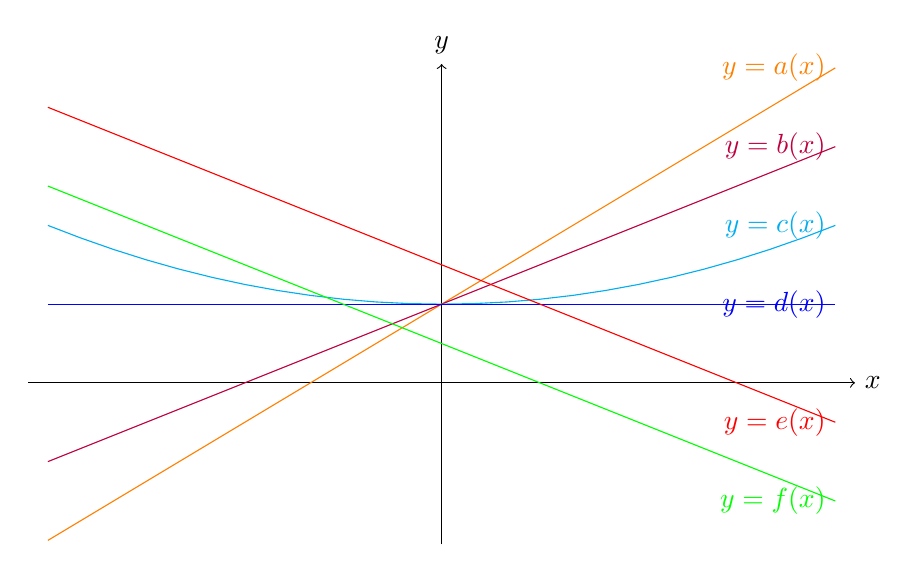
\begin{tikzpicture}[domain=-10:10, xscale=.5, yscale=0.1]
    \draw[->] (-10.5,0) -- (10.5,0) node[right] {$x$}; 
    \draw[->] (0,-20.5) -- (0,40.5) node[above] {$y$};
    \draw[color=orange] plot (\x,{3*\x + 10}) node[left] {$y=a(x)$};
    \draw[color=purple] plot (\x,{2*\x + 10}) node[left] {$y=b(x)$};
    \draw[color=cyan] plot (\x,{\x*\x/10 + 10}) node[left] {$y=c(x)$};
    \draw[color=blue]    plot (\x,10)       node[left] {$y=d(x)$}; 
    \draw[color=red]   plot (\x,{-2*\x + 15})    node[left] {$y=e(x)$}; 
    \draw[color=green] plot (\x,{-2*\x + 5}) node[left] {$y=f(x)$};
  \end{tikzpicture}
\end{center}

\subsection*{Ejercicio 4 (problema)}

Juan vende $1$ huevo $2$MXN y la comida de sus gallinas le cuesta $31$MXN cada día.
Expresar el dinero que gana cada día en funcíon del número de huevos $N$ que
vende. Trazar el gráfico par $0 \leq N \leq 20$ y deducir el mínimo de huevos
que debe vender para obtener un beneficio positivo. Comparar con la solución
de la ecuación lineal $2x - 31 = 0$.

\section{Soluciones de los ejercicios}

\subsection*{Ejercicio 1}

\begin{enumerate}
\item $x = -\frac{1}{2}$
\item $x = 5$
\item $x = -4$
\end{enumerate}

\subsection*{Ejercicio 2}

Las soluciones son dados por las interseciones de las rectas con el eje $X$.
$x_f = -\frac{1}{2}, x_g = 5, x_h = -4$. La recta de $f$ y $g$ son paralelas
por sus ecuaciones tienen el mismo $a = 2$. $-3 < 0$ y ${|-3|} < 2$ entonces
$h$ decrece y su pendiente es más importante que las dos otras rectas.

\begin{center}
  \begin{tikzpicture}[domain=-10:10, xscale=.5, yscale=0.1]
    \draw[->] (-10.5,0) -- (10.5,0) node[right] {$x$}; 
    \draw[->] (0,-40.5) -- (0,40.5) node[above] {$y$};
    \draw[color=blue]    plot (\x,2*\x+1)       node[left] {$y=f(x)$}; 
    \draw[color=red]   plot (\x,{2*\x -10})    node[left] {$y=g(x)$}; 
    \draw[color=green] plot (\x,{-3*\x - 12}) node[left] {$y=h(x)$};
    \foreach \x in {-10,...,10}
      \draw (\x,-1) --(\x,1) node[above] {$\x$};
    \foreach \y in {-40,-20,20,40}
      \draw (-.2, \y) --(.2, \y) node[right] {$\y$};
  \end{tikzpicture}
\end{center}

\subsection*{Ejercicio 3}

El gráfico de $c(x)=\frac{x^2}{10} + 10$ no es una recta.
$d(x) = 10$ es constante y coresponde a la recta paralela al eje $X$.
Las rectas de $a(x) = 3x+10$ y $b(x) = 2x+10$ intersectan el eje $Y$ en
$y = 10$ y la primera crece más rápido que la segunda porque $3 > 2$.
Las rectas paralelas son las de $e(x) = -2x+15$ y $f(x) = -2x+5$ y las
funciones son decreciendo (tienen el mismo $a=-2 < 0$). La primara recta está
ariba por que $15 > 5$.

\subsection*{Ejercicio 4 (problema)}

El beneficio es $B(N) = 2N - 31$MXN. Los puntos para $0 \leq N \leq 20$ están
sobre la recta de ecuación $y = 2x - 31$ y el beneficio es positivo para
$N \geq 16$. La solución del ecuación $2x - 31 = 0$ es
$x = \frac{31}{2} = 15.5$ y el mínimo de huevos es el más pequeño entero
$\geq 15.5$.

\begin{center}
  \begin{tikzpicture}[domain=-10:10, xscale=.5, yscale=.25]
    \draw[->] (0,0) -- (22,0) node[right] {$N$ (huevos)}; 
    \draw[->] (0,-35) -- (0,17) node[above] {$B(N)$ (MXN)};
    \foreach \N in {0,...,20}
      \draw (\N, 2*\N - 31) circle(.5);
    \foreach \N in {0,5,10,15,20}
      \draw (\N,-1) --(\N,1) node[above] {$\N$};
    \foreach \B in {-35,-30,-25,-20,-15,-10,-5,5,10,15}
      \draw (-.2, \B) --(.2, \B) node[right] {$\B$};
  \end{tikzpicture}
\end{center}
